%==================================================================================================
%   LUKES THESIS TEMPLATE 1.2
%   -------------------------
%   This template is based upon the offcial IMM PhD Thesis template, it is enhanced with a number
%   of new features and a number of errors have fixed. This template is intended to be complied to
%   PDF using PDFLATEX and is tested using the MiKTeX 2.9 LaTeX distribution.
%   It is based on the official DTU-IMM Thesis template by Finn Kuno Christensen in 2009.
%   Small bugfixes by Kasper Laursen in 2012 and 2013.
%   Small updates by Finn Kuno Christensen/Henning Christiansen in 2015.
%   -------------------------
%   Last Updated: 2015-01-08
%==================================================================================================
%
%==================================================================================================
% DOCUMENT SETUP
%==================================================================================================
\documentclass[10pt,twoside]{book}                  %Official DTU-IMM Thesis document setup
%
%Set to 'print' for printed version, use 'net' for online version
\def\thesisversion{print}
%
%==================================================================================================
% PACKAGES
%==================================================================================================
\usepackage{LukeThesis}                             %Import Thesis base style
\usepackage{hyperref}
\usepackage{listings}
\usepackage{float}
\usepackage{tabularx}
\usepackage{tikz}
\usepackage{alltt}
\usepackage{float}
\usepackage{todonotes}
\usepackage{url}
\usepackage{textcomp}
\usepackage{mathtools}
\usepackage{pdfpages}
\usepackage{amsmath}
\usepackage{pgfplots}
\usepackage{framed}
\usetikzlibrary{positioning}
\usetikzlibrary{backgrounds}
\definecolor{bblue}{HTML}{4F81BD}
\definecolor{rred}{HTML}{C0504D}
\definecolor{ggreen}{HTML}{9BBB59}
\definecolor{ppurple}{HTML}{9F4C7C}

%input{PhDMacros}                                   %Thesis specific macros
%
%==================================================================================================
% THESIS PROPERTIES (Modifiy these fields with your details)
%==================================================================================================
\def\thesisauthor{James Erik Groving Meade \\s173476}                     %Author
\def\thesistitle{Hardware Accelerator for the Training of Neural Networks}               %Title
\def\thesishandin{28-June}                       %Submission date (Day-Month}
\def\thesisdegree{M.Sc.}                              %Degree ('B.Eng', 'B.Sc.', 'M.Sc.' or 'PhD')
\def\thesisyear{2019}                               %Submission year
\def\thesisnumber{????}                             %DTU-IMM Serial number (do not include year)
\def\thesisISSN{0000-0000}                          %ISSN number
\def\thesiskeywords{FPGA, Hardware, Computer Architecture, Neural Networks}  %PDF keywords
\derivethesisprops                                  %Derive dependent properties
%
%==================================================================================================
% SECTION NUMBERING SETUP
%==================================================================================================
\setcounter{tocdepth}{2}                            %2 adds sections up to subsections
\setcounter{secnumdepth}{3}                         %Subsubsections get a number when this is 3
%
%==================================================================================================
% THESIS STRUCTURE  (Modifiy to include more chapters etc)
%==================================================================================================
\definecolor{mygreen}{RGB}{28,172,0} 
\lstset{language=Verilog, 
	captionpos=b,
	basicstyle=\small\ttfamily,   
	breaklines=true,
	morekeywords={},
	keywordstyle=\color{blue},
	morekeywords=[2]{1}, keywordstyle=[2]{\color{black}},
	identifierstyle=\color{black},
	commentstyle=\color{mygreen},
	showstringspaces=false,
	frame=single,
	numbers=left,
	tabsize=4,
	numberstyle={\small \color{black}},
	numbersep=9pt
}

\lstdefinelanguage{SystemVerilog}{
	keywords={always_ff, always_comb, if, begin, end, else, case, endcase, typedef, const, logic, integer, assign, parameter, localparam, module, posedge, negedge, enum, input, output, endmodule},
	keywordstyle=\color{blue}\bfseries,
	ndkeywords={\$display, \$itor, \$signed, ifdef, endif, class, export, boolean, throw, implements, import, this},
	ndkeywordstyle=\color{purple}\bfseries,
	identifierstyle=\color{black},
	sensitive=false,
	comment=[l]{//},
	morecomment=[s]{/*}{*/},
	commentstyle=\color{mygreen}\ttfamily,
	stringstyle=\color{mygreen}\ttfamily,
	%morestring=[b]',
	morestring=[b]"
}




\begin{document}
%------------------------
%Pre-frontmatter material
%------------------------
\prefrontmatter
%--------------------
%Frontmatter material
%--------------------
\frontmatter
\pagenumbering{roman}                               %Set frontmatter numbering style
\chapter{Abstract}

This thesis proposes a novel hardware architecture to accelerate the training of neural networks with small batch sizes. The accelerator uses a modular, parameterizable and computationally well-balanced design to successfully an implement high-performance online training of neural networks. By using parallelism at the neuron level, the accelerator was able to achieve a speedup of 17.3 against a PyTorch CPU implementation of a specific neural network architecture. The accelerator also performs nearly as fast as a PyTorch GPU implentation of the network that used a batch size of 50 during training.

This thesis also highlights the importance of high-precision calculation for training. The highest accuracy attained by the accelerator on the MNIST dataset was 85.845\%, which is a result of 18-bit fixed point precision being unable to successfully converge to a local optima due to the accumulation of precision error causing the degradation of training accuracy after a few epochs.

                                   %English summary of Thesis
\markboth{}{}                                       %Set headings (left)(right)
%\chapter{Summary (Danish)}
\begin{otherlanguage}{danish}

Målet for denne afhandling er at ...

\end{otherlanguage}                                   %Danish summary of Thesis
%\markboth{}{}                                       %Set headings (left)(right)
\chapter{Preface}

This thesis was prepared at DTU Compute in fulfilment of the requirements for acquiring an M.Sc. in Engineering.

The thesis deals with ...

The thesis consists of ...
%==================================================================================================
% SIGNATURE AREA
%==================================================================================================
\vspace{20mm}
\begin{center}
    \hspace{20mm} Lyngby, \thesishandin-\thesisyear
    \vspace{5mm}
    \newline
  %Update signature image file in line below
    
\includegraphics[scale=0.5]{figures/SignatureDummy}
\end{center}
\begin{flushright}
    \thesisauthor
\end{flushright}
% % % EOF % % %                                     %Preface
\markboth{}{}                                       %Set headings (left)(right)
\chapter{Acknowledgements}

First and foremost, I would like to sincerely thank my advisor Jens Sparsø for his time and guidance throughout the entire duration of my thesis. Our regular meetings helped me to stay grounded and to think critically about my project.

I would also like to thank my former classmate, Cheng Fu, who is currently a PhD student at the University of California, San Diego. My conversations with him at the beginning of my foray into this thesis helped me establish my footing.                            %Acknowledgements
\markboth{}{}                                       %Set headings (left)(right)
%------------------
% Table of contents
%------------------
\newpage\mbox{}\newpage
\chaptermark{Contents}
\pdfbookmark{\contentsname}{toc}
\renewcommand{\sectionmark}[1]{\markright{#1}}
\sectionmark{Contents}
\addtolength{\parskip}{-\baselineskip}
\tableofcontents
\addtolength{\parskip}{\baselineskip}
\renewcommand{\sectionmark}[1]{\markright{\thesection\ #1}}
%-------------
% Main content
%-------------
\mainmatter
\chapter{Introduction}
                                  %Chapter 1
\chapter{Background}
                                 	%Chapter 2
\chapter{Software Model}
\todo[inline]{figure for code snippets or nah?}
\section{Overview}
This section documents the general-purpose neural network framework that was written in C++ for this thesis. There is an example program that trains on the MNIST dataset and documents epoch-by-epoch training statistics. MNIST is a dataset of handwritten digits, containing 60,000 training images and 10,000 test images. The source code for the software model can be found in the appendix as well as online on github.\footnote{\url{
https://github.com/erikgroving/NeuralNetworkHardwareAccelerator/tree/master/SWModel}.}


\section{Motivation}
The software neural network framework was written so that the FPGA hardware model could be benchmarked against a CPU-based model that performs neural network inference and backward passes using the same method as the hardware model. This benchmark could be used to evaluate the performance of the hardware model. In addition, it could be benchmarked against professional open-source deep-learning frameworks that make use of advanced algebraic methods to perform computation such as matrix multiplication that inherently offer more efficiency. Furthermore, by developing a software model, the algorithmic integrity of the proposed network was able to verified and tested in an expedient manner by using a well-known testing framework, Google Test. Finally, if high floating-point precision were needed for training a network, then the software model could be used to learn the weights and parameters, and then subsequently be loaded into the weight BRAM of the FPGA hardware model.

\section{Design}
\subsection{Layers}
The software model was designed to be flexible such that any neural network architecture may be constructed so long as the layer types were implemented. The model currently supports 2D convolutional, fully connected, and pooling layers. 
\par 
All layers are derived from a base class, \texttt{Layer}. Certain methods such as \texttt{forward()} and \texttt{backward()} must be implemented by all derived classes. There is then a \texttt{Net} class that contains a \texttt{vector} of \texttt{Layer} objects. This allows for a flexible design, as one only need add layers to the \texttt{Net} object. Furthermore, the model can easily be extended to other layer types so long as the layer type derives from \texttt{Layer}. 
\par
The non-linear activation function used in the model is ReLU because the derivative is trivial to compute. Compared to the sigmoid function, ReLU is much more computationally feasible for an FPGA hardware implementation, and thereofre, ReLU was used in the software model so that both models would use the same activation function.
\subsection{Training}
\paragraph{The Softmax Function and Computing Loss Gradients}
The network uses an implicit Softmax function for the last layer since this converts the logits in the last layer to numbers that can be interpreted as probabilities, ideal for image classification. 
\par
The loss gradients for the neurons in the last layer are computed using multi-class cross entropy loss. Therefore, only one probability will account for loss, however, since each probability is an output from the softmax function which takes in all neuron outputs as input, all neurons in the last layer will have a loss gradient.
\par 
The derivative of this loss function is needed to perform backpropagation. We define $\mathcal{L}_i$ as the loss for neuron $i$ in the last layer and $z_i$ as the output of neuron $i$. We also introduce $y_i$, which is 1 if $x$ is an instance of class $i$ and 0 otherwise. We can then compute the loss gradient for neuron $i$ in the last layer quite simply as follows: 
\[    
\frac{\delta \mathcal{L}_i}{\delta z_i} = z_i - y_i
\]

\paragraph{Batch Size}
The software model supports batch training and thus a batch size is to be specified when creating an instance of a new network.
\paragraph{Learning Rate and Momentum}
The software model learns using stochastic gradient descent. As such, the network is configured with a learning rate and momentum. The learning rate may be manually readjusted during training epochs. Momentum is a learning technique in that previous updates to a parameter should impact the update in in a geometrically decreasing fashion. We first define a few parameters:
\begin{center}
    \begin{tabular} {r l}
    $m$  \hspace{12pt}---& the momentum parameter\\ 
    $v$  \hspace{12pt}---& `velocity' \\
    $lr$ \hspace{12pt}---& the learning rate \\
    $dx$ \hspace{12pt}---& the loss gradient for some weight or bias $x$. 
    \end{tabular}
\end{center}

The momentum-based update in the software model can then be mathematically represented in the following manner:
\begin{align*}
v &=  (m \times v) - (lr \times dx) \\
x &= x + v 
\end{align*}
We can observe that each time we update $x$, the previous updates update will have an effect, with the most recent updates having more effect than older ones. A typical value for momentum is 0.9.


\section{Source Code Structure}
The software model contains a Makefile and three folders: \textit{data}, \textit{src} and \textit{test}. The \textit{data} folder contains the MNIST binary data files, and is loaded by the example program that trains on the MNIST dataset. The \textit{src} folder contains the source code of the neural network framework. The \textit{test} folder contains test made using the Google Test C++ testing framework. The Makefile is used to build the source as well as tests. This section will detail the source files in the \textit{src} folder that are core to the software model framework. The files \textit{main.cpp} and \textit{parse\_data\{.cpp, .h\}} will be described in section \ref{sw-usage} that focuses on usage.

\paragraph{net\{.cpp, .h\}}
These files contain the definition of the \texttt{Net} class, the highest-level class of the network. After initializing a \texttt{Net} object, layers can be added to the neural network by calling the \texttt{addLayer()} method which will add a \texttt{Layer} object to a \texttt{vector}. The \texttt{Net} class also stores intermediate activations from the current inference, which are required when performing backward pass to calculate loss gradients. The key parameters to the \texttt{Net} object are set in its constructor, and are defined in table \ref{nettable}. 
\begin{table}
	\centering
	\begin{tabularx}{\textwidth}{|l|l|X|}
		\hline
		\textbf{Name} 			& \textbf{Type} 		& \textbf{Description} \\\hline
		\texttt{in}  			& \texttt{uint32\_t}	& Size of the input to the neural network.\\\hline
		\texttt{out}			& \texttt{uint32\_t}	& Size of the output of the neural network. \\\hline 
		\texttt{bs}				& \texttt{uint32\_t}	& Size of the batch size to be used when training the net.\\\hline 
		\texttt{lr}				& \texttt{double}	& The learning rate to be used during training of the network. Can be set and read using the functions \texttt{setLearningRate()} and \texttt{getLearningRate()}. \\\hline 
		\texttt{momentum}		& \texttt{double}	& The momentum to be used when performing updates to the weights and biases of the network.
		\\\hline
	\end{tabularx}
	\caption{Description of parameters for the constructor \texttt{Net} class.}
	\label{nettable}
\end{table}
\par 
The \texttt{Net} class has a method \texttt{inference()} that computes the forward pass for a batch of inputs, thus the argument is a 2-d \texttt{vector}, with each outer index corresponding to an input. The \texttt{()} operator has also been overloaded to call \texttt{inference()}. This is all that is needed to compute a forward pass.
\par 
To compute the backward pass, \texttt{computeLossAndGradients()} should be called first. This method takes in the label data as a \texttt{vector} for the inputs as an argument and computes the loss gradients for the outer layer of the network. Next, a call to \texttt{backpropLoss()} should be made; this method propagates the outer layer loss gradients back through the neural network. After the loss has been back-propagated, weights of each \texttt{Neuron} in the network should be updated by calling \texttt{update()}. Previously cached forward pass activation data should then be cleared with a call to \texttt{clearSavedData()}.
\paragraph{layer.h}
This file contains the \texttt{Layer} class, which serves as the base class for all the different types of layer classes in the framework. It contains virtual methods \texttt{forward()} and \texttt{backward()}, representing the forward and backward pass functionality that must be implemented. All layer classes must also contain a \texttt{getType()} method to identify the layer type, as well as methods for \texttt{updateWeights()}, \texttt{clearData()}, and \texttt{getOutput()}.

\paragraph{convolutional\{.cpp, .h\}}
These files contain the definition of the \texttt{ConvLayer} class, which implements a 2D-convolutional layer, and derives from the \texttt{Layer} class. A unique method to the \texttt{ConvLayer} class is the \texttt{getWindowPixels()} method, which returns the pixels inside the filter window, and is used when computing both the forward and backward passes.  The class' constructor and key parameters are described in table \ref{convtable}.
\begin{table}
\centering
\begin{tabularx}{\textwidth}{|l|l|X|}
	\hline
	\textbf{Name} 			& \textbf{Type} 		& \textbf{Description} \\\hline
	\texttt{dim}  			& \texttt{uint32\_t}	& Dimensions of the input. The dimension is assumed square, meaning that rows = \texttt{dim} and columns = \texttt{dim}.\\\hline
	\texttt{filt\_size} 	& \texttt{uint32\_t}	& Dimension of the filter used for the convolution, dimension also assumed square. \\\hline 
		\texttt{stride} 	& \texttt{uint32\_t}	& Size of the stride \\\hline 
	\texttt{padding} 		& \texttt{uint32\_t}	& Padding used for convolution. \\\hline 
	\texttt{in\_channels} 	& \texttt{uint32\_t}	& Amount of channels in the input. \\\hline 
	\texttt{out\_channels} 	& \texttt{uint32\_t}	& Amount of channels in the output. \\\hline
\end{tabularx}
\caption{Description of parameters for the \texttt{ConvLayer} class.}
\label{convtable}
\end{table}


\paragraph{fullyconnected\{.cpp,.h\}}
These files define the \texttt{FullyConnected} class. The class only has two defining parameters in its constructor: \texttt{in} and \texttt{out}, which are of type \texttt{uint32\_t} and specify the input and output size to the layer, respectively. It derives from the base \texttt{Layer} class, so methods such as \texttt{forward()} and \texttt{backward()} are also implemented.

\paragraph{pooling\{.cpp,.h\}}
These files define the \texttt{PoolingLayer} class. The class derives from \texttt{Layer} and performs a 2D 2$\times$2 max pooling operation. There are three main parameters for the class: \texttt{dim\_i}, \texttt{dim\_o}, and \texttt{channels}. The parameters \texttt{dim\_i} and \texttt{dim\_o} specify the dimension of the input and output feature vectors. Since the layer currently only performs 2$\times$2 max pooling, \texttt{dim\_o} will always be half of \texttt{dim\_i}, though if different types of pooling filters were to be supported, then \texttt{dim\_o} would be necessary. The \texttt{channels} parameter is used to specify the number of channels of size \texttt{dim\_i} $\times$ \texttt{dim\_i} present in the input.

\paragraph{neuron\{.cpp, .h\}}
These files define the \texttt{Neuron} class. The \texttt{Neuron} class is the computational building block of the fully connected and convolutional layers. The fan-in of the neuron is specified in the constructor. Weights should be initialized using the \texttt{initWeights()} method, which implements He initialization \cite{HeZR015}. He initialization randomly initializes weights using a normal distribution with a mean of 0 and a variance of $\frac{2}{\text{fan\_in}}$. 
\par 
The class implements all necessary computational elements for a neuron in a neural network. During a forward pass, a neuron's net and activation are computed with \texttt{computeNet()} and \texttt{computeActivation()} respectively. When computing the backward pass, the gradients for the neuron's weights are computed using \texttt{calculateGradient()}. Weights can be subsequently updated using the \texttt{updateWeights()} function. Finally, all gradient data can be cleared using \texttt{clearBackwardData()}.

\section{Usage}\label{sw-usage}
This section will show how the software model may be used for image classification. In the following example, the software model will be trained to classify handwritten digits from the MNIST database. Each image is a handwritten digit of size 28$\times$28. The relevant files specific to this example are \textit{main.cpp} and \textit{parse\_data.cpp}.
\paragraph{Load the Training and Testing Data}
The first step to any neural network problem is to load the training and testing dataset.
The MNIST dataset is provided as binary files and helper functions to load the data have been provided in \textit{parse\_data.cpp}. Training and testing data can be loaded as shown below.
\begin{lstlisting}[language=c++]
std::vector< std::vector<double> > trainX;
std::vector<int> trainY;
std::vector< std::vector<double> > testX;
std::vector<int> testY;
trainX = readImages("data/train-images.idx3-ubyte");
trainY = readLabels("data/train-labels.idx1-ubyte");
testX = readImages("data/t10k-images.idx3-ubyte");
testY = readLabels("data/t10k-labels.idx1-ubyte");
\end{lstlisting}
\paragraph{Create a \texttt{Net} Instance}
The next step is to create a \texttt{Net} object with the relevant hyperparameters to be used for the neural network. The below code accomplishes this.
\begin{lstlisting}[language=c++]
int 	input_size  = 28*28;
int     output_size = 10;
int     batch_size  = 200;
double  momentum    = 0.9;
double  lr          = 0.01; 
Net net(input_size, output_size, batch_size, lr, momentum);
\end{lstlisting}

\paragraph{Create Layer Objects and Add them to the \texttt{Net} Object} 
After the \texttt{Net} object has been created, layers need to be added to the network. Two configuration options are present in \textit{main.cpp}; one implements a 7-layer convolutional neural network, and the other implements a 4-layer fully connected neural network. The below code snippet shows how the 7-layer convolutional neural network is implemented. The software model was designed with simplicity in mind, so the below code is relatively straightforward to follow.
\begin{lstlisting}[language=c++]
Layer* conv1 = new ConvLayer(28, 3, 1, 1, 1, 8);
Layer* pool1 = new PoolingLayer(28, 14, 8);
Layer* conv2 = new ConvLayer(14, 3, 1, 1, 8, 16);
Layer* pool2 = new PoolingLayer(14, 7, 16);
Layer* fc1 = new FullyConnected(16*7*7, 64);
Layer* fc2 = new FullyConnected(64, 10);

net.addLayer(conv1);
net.addLayer(pool1);
net.addLayer(conv2);
net.addLayer(pool2);
net.addLayer(fc1);
net.addLayer(fc2);
\end{lstlisting}

\paragraph{Train the Net}
In \textit{main.cpp}, a function \texttt{trainNet()} has been implemented, which trains the net using batch training. The actual training for a given batch only requires 5 lines of code, and is shown below.
\begin{lstlisting}[language=c++]
net(in_batch);
net.computeLossAndGradients(out_batch);
net.backpropLoss();
net.update();
net.clearSavedData();
\end{lstlisting}
\paragraph{Build and Run the Model}
Compile the code by running \texttt{make} in the \textit{SWModel} directory. The model will then train for the amount of epochs specified in the call to the \texttt{trainNet()} function in \texttt{main()}. Since the model is initialized with random weights, the final result of training is non-deterministic. Output similar to the output shown in figure \ref{sw-model-output} can be expected. In this case, the fully connected model was used, and train to a maximum accuracy of 97.62\%. it is also worth noting the expected differences in loss and accuracy between the training and test datasets. This discrepancy is expected as the network never learns from the test dataset.
The difference between test and training dataset accuracy is normally used to quantify how well the network is able to generalize from the training dataset.
\begin{figure}
\begin{lstlisting}
Running software model...
Starting Accuracy
Total correct: 1022 / 10000
Accuracy: 0.1022

Epoch: 0
--- Training Stats ---
Total correct: 54914 / 60000
Accuracy: 0.915233
Loss: 0.290908
--- Test Stats ---
Total correct: 9183 / 10000
Accuracy: 0.9183
Loss: 0.280574

Epoch: 1
--- Training Stats ---
Total correct: 56213 / 60000
Accuracy: 0.936883
Loss: 0.218062
--- Test Stats ---
Total correct: 9390 / 10000
Accuracy: 0.939
Loss: 0.214584

...

Epoch: 36
--- Training Stats ---
Total correct: 59168 / 60000
Accuracy: 0.986133
Loss: 0.0516957
--- Test Stats ---
Total correct: 9762 / 10000
Accuracy: 0.9762
Loss: 0.0845137
\end{lstlisting}
\caption{An expected output from using the software model on the provided MNIST dataset. Epochs 2-35 omitted for brevity. In this training run, the network reached a maximum test set accuracy of 97.62\%.}
\label{sw-model-output}
\end{figure}

\section{Testing}
To ensure the correctness of the software model, several test suites were created during development. Source code for the test suites can be found in the \textit{test} folder as well as in the appendix.
\todo[inline]{source code in appendix}
\subsection{Test Suites}
Four test suites were created during the development of the software model. The test cases were written to test features as they were developed. As such, the tests include neuron functionality, forward pass for fully connected and convolutional layers, and finally a gradient checking test suite to verify the backward pass. This section elaborates on the test suites that were used during development.

\paragraph{Neuron Testing}
The neuron test suite, found in \textit{neuron\_test.cpp}, contains one primary test case that sets the weights of a neuron, computes the activation, and verifies that the activation is correct.

\paragraph{Fully Connnected Forward Pass}
The test case for a fully connected layer's forward pass is located in \textit{fullyconnected\_test.cpp}. The test case creates a \texttt{FullyConnected} layer that has 3 inputs and 4 outputs. The weights are then set and an input is sent forward through the layer. Each of the 4 outputs are then verified to be correct.

\paragraph{Convolutional Forward Pass}
There is a test case to verify the convolutional forward pass located in \textit{conv\_test.cpp}. The test creates a convolutional layer that takes a 2$\times$2 feature vector with 2 channels, uses a 3$\times$3 filter for convolution, uses a stride and padding of 1, and produces 2 output channels. Weights and inputs were the arbitrarily assigned and the forward pass was computed and verified against the output that had been previously calculated manually.

\paragraph{Gradient Checking}
It would be very tedious and error-prone to debug the backward pass of a neural network using manual calculations, thus the general standard method of testing the gradients computed during a backward pass is to use gradient checking. Note that during the backward pass, all the loss gradients for every single weight and bias are calculated. For every weight (and bias), the partial derivative $\frac{\delta \mathcal{L}}{\delta w_i}$ is computed. Gradient checking verifies that the mathematically computed analytic derivative aligns with a numerically estimated derivative \cite{grad-check-stanford}. The numerical gradient can be computed as follows:
\begin{align*}
	\frac{\delta \mathcal{L}(w_i)}{\delta w_i} = \frac{\mathcal{L}(w_i + \epsilon) - \mathcal{L}(w_i - \epsilon)}{2\epsilon}
\end{align*}
The partial derivative of the loss with respect to a certain weight $w_i$ can thus be estimated by calculating the loss after incrementing $w_i$ by a small $\epsilon$, calculating the loss after decrementing $w_i$ by $\epsilon$, and then dividing the difference by $2\epsilon$. As long as $\epsilon$ is rather small, the derivatives should be near exact. In these test cases, $\epsilon = 10^{-4}$. Once we have the analytic and numerical gradient, we can compute the relative error as shown below:
\begin{align*}
	\text{Relative gradient error} = \frac{\lvert\mathcal{L}'(w_i)_a - \mathcal{L}'(w_i)_n\rvert}
		{\max \;\left(\lvert\mathcal{L}'(w_i)_a\rvert,\; \lvert\mathcal{L}'(w_i)_n\rvert\right)}
\end{align*}
If the relative error is below a certain threshhold, then it is safe to assume the gradient has been calculated correctly. In this test suite, the relative error threshhold must be lower than $10^{-7}$.
\par 
The two test cases in \textit{gradient\_check\_test.cpp} perform gradient checks for a fully connected network and for a convolutional neural network. The fully connected network gradient check test creates a neural network with an architecture shown in figure \ref{fctest}.
\begin{figure}
	\begin{lstlisting}[language=C++]
int 	input_size  = 100;
int 	output_size = 2;
int 	batch_size  = 1;
double 	momentum    = 0.9;
double 	lr          = 0.001; 
Net net(input_size, output_size, batch_size, lr, momentum);


Layer* fc1 = new FullyConnected(input_size, 98);
Layer* fc2 = new FullyConnected(98, 64);
Layer* fc3 = new FullyConnected(64, output_size);

net.addLayer(fc1);
net.addLayer(fc2);
net.addLayer(fc3);		
	\end{lstlisting}
	\caption{Layer created for the fully connected gradient check test.}
	\label{fctest}
\end{figure}
\par
The test then creates 10 random inputs, each having a random label. Each input sample is fed forward through the network and analytic gradients are computed for each weight. The numerical gradient is then subsequently computed for a random weight. The random weight can belong to any neuron and any layer. This process of choosing a random weight, calculating the numerical gradient, comparing it to the analytic gradient is then repeated 100 times. The test asserts that the relative error is less than $10^{-7}$ each time. A portion of the computed analytic and numerical gradients are shown in figure \ref{num-grads}.
\begin{figure}
	\begin{lstlisting}
Layer: 2, Neuron: 0,  Weight: 31 
Analytic Gradient: -0.0638284 Numerical Gradient: -0.0638284

Layer: 0, Neuron: 93, Weight: 71 
Analytic Gradient: -0.156235  Numerical Gradient: -0.156235

Layer: 1, Neuron: 34, Weight: 29 
Analytic Gradient: -1.22615   Numerical Gradient: -1.22615

Layer: 1, Neuron: 12, Weight: 43 
Analytic Gradient: 0.376021   Numerical Gradient: 0.376021		
	\end{lstlisting}
	\caption{Results from the fully connected test using randomly sampled weights to perform gradient checking}
	\label{num-grads}
\end{figure}

The convolutional gradient checking test is set up in the same manner as the fully connected gradient checking test, except that the network structure is different. The network is now a \textbf{convolutional layer --- pooling layer --- convolutional layer --- fully connected layer}. The input is randomized 8x8 data, and convolutional layers use 3$\times$3 filters with a padding and stride set to 1. The first convolutional layer has 3 output channels and the second convolutional layer has 3 input channels and 6 output channels. The code used to create the network is shown in figure \ref{conv-net}.

\begin{figure}
	\begin{lstlisting}[language=C++]
int    input_size   = 8*8;
int    output_size  = 2;
int    batch_size   = 1;
double momentum     = 0.9;
double lr           = 0.001; 
Net net(input_size, output_size, batch_size, lr, momentum);

Layer* conv1 = new ConvLayer(8, 3, 1, 1, 1, 3);
Layer* pool1 = new PoolingLayer(8, 4, 3);
Layer* conv2 = new ConvLayer(4, 3, 1, 1, 3, 6);
Layer* fc1   = new FullyConnected(4*4*6, output_size);

net.addLayer(conv1);
net.addLayer(pool1);
net.addLayer(conv2);
net.addLayer(fc1);	
	\end{lstlisting}
	\caption{Layer created for the convolutional layer gradient check test.}
	\label{conv-net}
\end{figure}


\subsection{Building and Running the Test Suites}
The test suites requires Google Test to compile. Google Test can be downloaded online at github \footnote{\url{https://github.com/google/googletest}}. The \textit{googletest} directory should then be placed under the \textit{SWModel} folder. The test suite can then be compiled using the provided Makefile and the following command:
\begin{lstlisting}
> make all_tests
\end{lstlisting}
This will produce an executable in the \textit{SWModel} directory called \textbf{all\_tests}. The test suites can be run by invoking the executable. The output is shown in figure \ref{goog-out}
\begin{figure}

\begin{framed}
\begin{alltt}
> ./all\_tests
Running main() from ./googletest/src/gtest\_main.cc
{\color{mygreen}[==========]} Running 6 tests from 4 test cases.
{\color{mygreen}[----------]} Global test environment set-up.
{\color{mygreen}[----------]} 1 test from ConvTest
{\color{mygreen}[ RUN      ]} ConvTest.TestForward
{\color{mygreen}[       OK ]} ConvTest.TestForward (1 ms)
{\color{mygreen}[----------]} 1 test from ConvTest (11 ms total)

{\color{mygreen}[----------]} 1 test from FCTest
{\color{mygreen}[ RUN      ]} FCTest.TestForward
{\color{mygreen}[       OK ]} FCTest.TestForward (0 ms)
{\color{mygreen}[----------]} 1 test from FCTest (10 ms total)

{\color{mygreen}[----------]} 2 tests from NeuronTest
{\color{mygreen}[ RUN      ]} NeuronTest.InitWeights
{\color{mygreen}[       OK ]} NeuronTest.InitWeights (0 ms)
{\color{mygreen}[ RUN      ]} NeuronTest.SetWeightsAndGetOutput
{\color{mygreen}[       OK ]} NeuronTest.SetWeightsAndGetOutput (0 ms)
{\color{mygreen}[----------]} 2 tests from NeuronTest (29 ms total)

{\color{mygreen}[----------]} 2 tests from GradientTest
{\color{mygreen}[ RUN      ]} GradientTest.FCGradientCheck
{\color{mygreen}[       OK ]} GradientTest.FCGradientCheck (950 ms)
{\color{mygreen}[ RUN      ]} GradientTest.ConvGradientCheck
{\color{mygreen}[       OK ]} GradientTest.ConvGradientCheck (2260 ms)
{\color{mygreen}[----------]} 2 tests from GradientTest (3223 ms total)

{\color{mygreen}[----------]} Global test environment tear-down
{\color{mygreen}[==========]} 6 tests from 4 test cases ran. (3329 ms total)
{\color{mygreen}[  PASSED  ]} 6 tests.
\end{alltt}
\end{framed}
\caption{Test coverage output using the Google Test C++ testing framework to verify the correctness of the software model for both forward and backward passes.}
\label{goog-out}
\end{figure}

                                  %Chapter 3
\chapter{Hardware Model and Implementation}

This chapter details the hardware designed during this Master's thesis to accelerate neural network training. The current hardware implements both training and inference acceleration for the neural network architecture described in section \ref{net-arch}.
\todo[inline]{Refer to github, appendix, and project link}
\section{Specifications}
The hardware model was implemented using a ZedBoard. The ZedBoard is a development board equipped with a Zynq-7000 XC7Z020 SoC. The Zynq series has both a processing system and programmable logic, where the processing system is a ARM Cortex-A9 based processor (hereafter referred to as the ``PS'') and the programmable logic is an Artix-7 series FPGA. Bitstreams for the FPGA were generated using Vivado 2018.3 and PetaLinux boot images for the PS were created using Xilinx SDK. The hardware description language (HDL) code for the project was primarily written in SystemVerilog. The programs run on the PS were written in C.
\todo[inline]{Cite the datasheets}

\section{The Implemented Neural Network}\label{net-arch}
\todo[inline]{MACs of the networks, distribution of kernels, probably to go in analysis}
\todo[inline]{figure of network.}

\section{Design Goals}
There were a few key principles that guided the overall design process throughout the development of the hardware accelerator. A core tenet was to maintain the project such that in the future HDL could be generated for training a network of any architecture so long as the desired layer types had an implementation. As a result, all layers have been modularized and internal components are parameterized. Designing in a modular and parameterizable fashion also allows for quick and easy readjustments to the neural network architecture if needed.
\par 
In addition, optimal usage of resources available was prioritized. For example, the limiting FPGA resource was the amount of digital signal processing slices (DSPs). Therefore, the FPGA design optimized the distribution of DSPs over other resources as opposed to saving an extra Block RAM (BRAM) block. 

\section{Overall Architecture}
In the hardware model, both the Zynq's PS and the FPGA were used to facilitate a cohesive and efficient architecture to accelerate neural network computation. The 

\section{Layer Architecture}
\subsection{Fully Connected Layers}
\subsection{Softmax Layer}
To have training be feasible, a proper loss function was required to calculate initial gradients for the output neurons. As such, cross entropy loss, one of the most popular loss functions in deep learning was chosen for this network. Cross-entropy loss is a statistical loss that uses probabilities as input, as shown below.
\begin{align}
\mathcal{L}(y) = - \sum_{i = 1}^{C}y_{i,c}\log(p_{i,c})
\end{align}
In this equation, 
\todo[inline]{Consider against the cross entropy loss defined in chapter 3, define it in chapter 2 IMO}

As explained in chapter \ref{background}, the softmax functions converts logits to probabilities in following manner

\section{Interlayer Architecture}
\section{ARM-Zynq Communication}
\section{Memory Map Layout}
\section{Project Structure}


\begin{figure}
	\begin{tikzpicture}[]
	\node[] at (0,0) (top) {neural\_net\_top.sv};
	\node[] at (3, -1) (mlled) {fc0\_layer.sv};
	\node[] at (3, -2) (debounce) {debounce.v};
	\node[] at (3, -3) (scope) {red\_pitaya\_scope.v};
	\node[] at (3, -4) (buffermodule) {buffer\_module.v};
	\node[] at (3, -5) (irf) {internal\_ref\_gen.xci};
	\node[] at (3, -6) (pfd) {pfd.v};
	\node[] at (6, -7) (pfdblock) {pfd\_block.v};
	\node[] at (6, -8) (pfdfilter) {pfd\_filter.v};
	\node[] at (3, -9) (freqcounter) {freq\_counter.v};
	\node[] at (6, -10) (freqcounterblock) {freq\_counter\_block.v};
	\node[] at (9, -11) (interp) {freq\_interp\_clk.xci};
	\node[] at (3, -12) (pid) {red\_pitaya\_pid.v};
	\node[] at (6, -13) (pidblock) {imra\_pid\_block.v};
	\node[] at (6, -14) (pidfilt) {iir\_filter.v};
	\node[] at (3, -15) (analog) {red\_pitaya\_analog.v};
	\node[] at (6, -16) (dds) {dds/mixer/lpf};
	
	
	\draw [->] (top) |- (mlled.west);
	\draw [->] (top) |- (debounce.west);
	\draw [->] (top) |- (scope.west);
	\draw [->] (top) |- (buffermodule.west);
	\draw [->] (top) |- (irf.west);
	\draw [->] (top) |- (pfd.west);
	\draw [->] (top) |- (freqcounter.west);
	\draw [->] (top) |- (pid.west);
	\draw [->] (top) |- (analog.west);
	\draw [->] (pfd) |- (pfdblock.west);
	\draw [->] (pfd) |- (pfdfilter.west);
	\draw [->] (freqcounter) |- (freqcounterblock.west);							
	\draw [->] (freqcounterblock) |- (interp.west);
	\draw [->] (pid) |- (pidblock.west);
	\draw [->] (pid) |- (pidfilt.west);
	\draw [->] (analog) |- (dds.west);
	
	
	
	\end{tikzpicture}
	\caption{Hierarchy of the FPGA code used for the implementation of the network.}
\end{figure}                                  %Chapter 4
\chapter{Hardware Model Testing and Verification}\label{hw-model-testing}
Verification is a vital part of hardware design. For this project, all relevant functionality in the FPGA was verified by simulation.
\section{Simulation}
During FPGA development, four different testbenches were created to test the functionality of the design. The first three were module level testbenches to test the scheduler, fully-connected layer, and softmax layers. The fourth testbench tests the entire FPGA design, thus verification of the fourth testbench means that all modules are functional. Therefore, this section will discuss verification of the fourth testbench, which is a full test of the network: \texttt{neural\_net\_top\_tb.sv}, found in the directory \textit{FPGA/FPGA.srcs/sim\_1/new} of the GitHub repository as well as in Appendix \ref{app:hw}.

\subsection{Project Modifications to Simulate of the Design}
To conduct the full-scale test of the network, an input needed to be provided to the network on which to perform training. This was done by using a BRAM to store a random input generated by the same Python script (\texttt{weight\_coeff.py}) used to generate the weights for the weight BRAMS. When the simulation runs, the input to the network comes from this input BRAM rather than from the PS.

\subsection{Testing Environment}
The Vivado Simulator was used to perform simulation of the hardware. The testbench was run through Vivado's Tcl shell. During the testing process, a simulation would be ran and then diagnostic data in a test file could be  The below commands run from the Vivado Tcl show how to open the project, run the testbench for 50000 ns, and have all output written to a file.
\begin{lstlisting}
Vivado% open_proj FPGA.xpr
Scanning sources...
Finished scanning sources
open_project: Time (s): cpu = 00:00:11 ; elapsed = 00:00:13 . Memory (MB): peak = 322.016 ; gain = 71.828
Vivado% launch_simulation > sim_out
Vivado% run 50000 >> sim_out
\end{lstlisting}

\subsection{Simulation Output}
Verification and debugging was simple through the use of informative simulation output files. The project formatted signal data to be easy to read through the use of \texttt{\$display} statements. An example of this is shown in listing \ref{display-list}. This example is from \texttt{neural\_net\_top.sv} and prints the current cycle number and FC2 output and gradient data; \texttt{sf} and \texttt{sf2} are scaling factors for activations and gradients, respectively. These scaling factors allow the fixed-point Q format values to be displayed as their floating point equivalent. These types of display statements are ubiquitous in the modules of the project. Once verified, most of these display statements were commented out to prevent clutter of the simulation output file.
\begin{lstlisting}[
caption={Example debug code for simulating the functionality of the hardware model}, label={display-list}, language=SystemVerilog, upquote=true]
`ifdef DEBUG
integer clk_cycle;
integer it;

always_ff @(posedge clk) begin
  if (reset) begin
    clk_cycle   <= 0;
  end
  else begin
    clk_cycle   <=  clk_cycle + 1'b1;
  end
  $display("\n\n------ CYCLE %04d ------", clk_cycle);
  	
  $display("---FC2 GRADIENTS---");    
  $display("img_label: %d", img_label);    
  for (it = 0; it < `FC2_NEURONS; it = it + 1) begin
    $display("%02d:\t%f", it, 
      $itor($signed(fc2_gradients[it])) * sf2);
  end
  
  $display("--- FC2 OUT ---");        
  $display("fc2_buf_valid: %01b" , fc2_buf_valid);
  for (it= 0; it < `FC2_NEURONS; it=it+1) begin
    $display("%02d: %f", it, 
      $itor($signed(fc2_act_o_buf[it])) * sf); 
  end
end 
`endif    
\end{lstlisting}

With this output redirected to a text file, signal data per cycle can be easily found. Furthermore, jumping to a previous or next cycle is quick. For example, in Vim, this can be done with by pressing `N' or `n', respectively. This method of debugging with Vim is shown in Figure \ref{vim-out}, displaying the output generated from the code in Listing \ref{display-list}.
\begin{figure}
	\centering 
	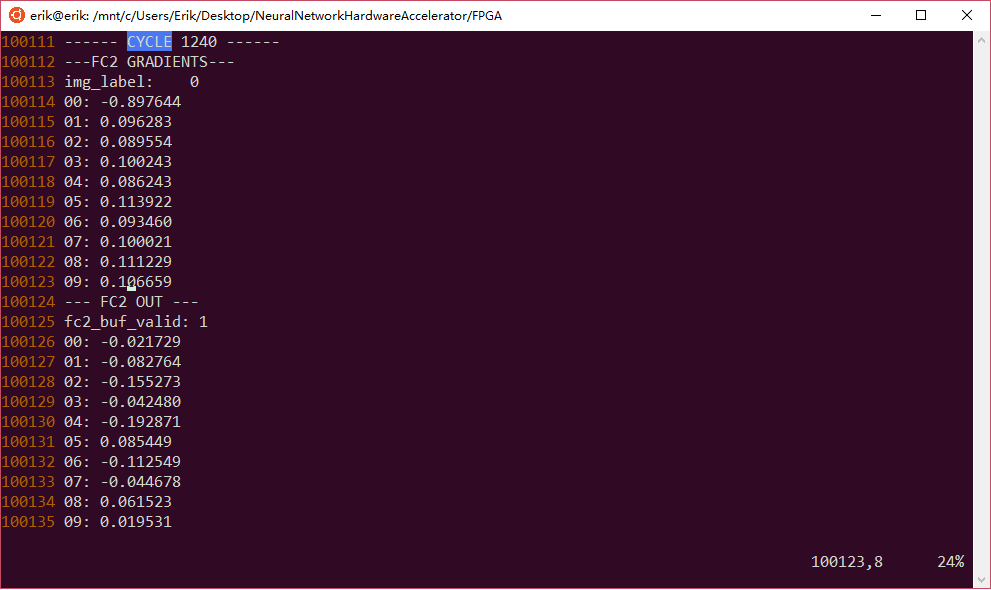
\includegraphics[width=\textwidth]{figures/vim_output}
	\caption{Jumping from cycle to cycle to view debugging data using Vim}\label{vim-out}
\end{figure}

\subsection{Correctness of Simulated Outputs}
A Python script was written to aid in verification of the hardware simulation. This script, \texttt{fpga\_forward\_backward\_pass\_test.py}, is located in Appendix \ref{app:hw-test} as well as in the \textit{misc} folder of the project on GitHub.

This script parses the Xilinx coefficient files for the input to the network, as well as for all the neurons in all the layers and converts them to floating point numbers. The script then performs the forward pass using the parsed weights and prints the outputs. The script then computes the backward pass and also prints out all neuron and weight gradients. The hardware model can then be verified by checking that the outputs at each stage of computation align with the Python script. Note that values are not compared for equality, but for relative correctness, since the Python script uses floating point and the hardware model uses 18-bit fixed point.

Furthermore, to ensure that the script's computed outputs and gradients are correct, the script also implements gradient checking tests for itself. With this assurance,  the script's computed output and gradients were successfully verified as correct and thus could be used as a baseline against which to compare the hardware model. Note that the gradient check testing for the testing script was based on the gradient checks implemented for the software model in Chapter \ref{ch-sw-model}, and example gradient check tests are shown in Listing \ref{py-grad-check}.

\begin{lstlisting}[
caption={Gradient checks for randomly chosen weights in the Python verification script that uses inputs and weights read from the Xilinx coefficient files of the BRAMs in the hardware model. Only three non-zero gradients shown for brevity.}, label={py-grad-check}, language=SystemVerilog, upquote=true]
> python3 fpga_forward_backward_pass_test.py
../FPGA/FPGA.srcs/sources_1/ip/fc0_weights_1.17.coe
../FPGA/FPGA.srcs/sources_1/ip/fc1_weights2_1.17.coe
../FPGA/FPGA.srcs/sources_1/ip/fc2_weights_1.17.coe
Calculated gradient:    -0.003531676695546401
Numerical gradient:     -0.003531676693313557

Calculated gradient:    -0.006374946805618298
Numerical gradient:     -0.0063749433798498956

Calculated gradient:    0.0006677415295515585
Numerical gradient:     0.0006677441533042838
\end{lstlisting}

\paragraph{Forward Pass Verification}
The Python script was used to verify the correctness of the forward pass of the FPGA layer by layer. Forward pass layer outputs for softmax layer from the simulation and script are compared side-by-side in Listing \ref{sm-forward}. Since the softmax output depends on the outputs from FC0, FC1, and FC2, these layer outputs are not shown for the sake of space. From these tests, the simulated forward pass outputs of the hardware model are shown to be correct. The full outputs for every layer may be seen in the \textit{HW\_Verification} folder of the GitHub repository.

\begin{lstlisting}[
caption={Softmax output. All 10 Neuron outputs shown.}, label={sm-forward}, language=SystemVerilog, upquote=true, numbers=none]
SIMULATION                  PYTHON SCRIPT
Neuron		Activation      Neuron		Activation
00			0.102348        0			0.10235213231346099
01			0.096283        1			0.09627338472902423
02			0.089554        2			0.08953177512141873
03			0.100243        3			0.1002532810000227
04			0.086243        4			0.08622264587243636
05			0.113922        5			0.11397991662882098
06			0.093460        6			0.09343919203092571
07			0.100021        7			0.10005157131620508
08			0.111229        8			0.11123918032286678
09			0.106659        9			0.10665692066481845
\end{lstlisting}

\paragraph{Backward Pass Verification}
The backward pass was verified in the same way as the forward pass, though there are many more gradients than outputs. There is 1 gradient for each neuron and weight, totalling over 80,000 gradients. The forward pass outputs and backward pass gradients can be seen in their entirety in the \textit{hardware\_verification} folder of the GitHub repository.

The gradients in the backward pass all stem from the output layer gradients which come from the softmax function. The steps for deriving the gradients of the output layer is a softmax based neural network are explained in more detail in Chapter \ref{background}, though the gradients are essentially the softmax output visible in Listing \ref{sm-forward} except that the neuron representing the inputs class label is subtracted by 1. 

Listing \ref{rand-weight-gradients} shows randomly selected weight gradients from each of the fully-connected layers. The weight gradients depend on the neuron gradients, thus the neuron gradients for that layer must be correct for the weight gradients to be correct; because of this, only weight gradients are shown in the figure, though neuron gradients are also available for viewing in the \textit{hardware\_verification} folder. As can be seen, the gradients are calculated to relatively high accuracy. This level of accuracy is directly correlated to the fact that the gradients are all Q1.17, maximizing the amount of fractional bits. Note that the 1 integer bit is required to represent the output layer gradient (since the input class label neuron is subtracted by 1), so the radix cannot be moved any further.


\begin{lstlisting}[
caption={5 randomly selected weight gradients from each of the fully connected layers}, label={rand-weight-gradients}, language=SystemVerilog, upquote=true, numbers=none]
SIMULATION                  PYTHON SCRIPT
FC0
Neuron	Weight	Gradient	Neuron	Weight 	Gradient
09 		593 	0.000763    09   	593 	0.00076932259
19 		711 	0.006874    19 		711	 	0.00688892029
37 		412    -0.006149    37  	412    -0.00613842723
57 		128 	0.000610    57  	128 	0.00061567956
74 		485    -0.000282    74  	485    -0.00027281649

FC1
Neuron	Weight	Gradient	Neuron	Weight 	Gradient
02 		051    -0.003815    02   	051    -0.00380934976
19 		097    -0.019463    19  	097    -0.01948172921
24 		035    -0.013214    24  	035    -0.01325251269
37 		094 	0.016045    37  	094  	0.01610831241
51 		030 	0.016563    51  	030  	0.01659535729

FC2
Neuron	Weight	Gradient	Neuron	Weight 	Gradient
01  	043 	0.015907    01 		043 	0.01595727359
03  	002 	0.016861    03 		002  	0.01688975169
04  	057 	0.005745    04 		057 	0.00578264697
08  	023 	0.024437    08 		023 	0.02451471064
09  	024 	0.000542    09 		024 	0.00055094484
\end{lstlisting}
                                  %Chapter 5
\chapter{Results}\label{results}
\section{Benchmarking Models and Structure}
Some of the results in this chapter are based on evaluating the hardware model (HWM) against other models implementing the same neural network. The other models include my software model (SWM), PyTorch running on the CPU (PyCPU), and PyTorch running on the GPU (PyGPU). My software model performs the same computations as the hardware model, so this provides insight to speedup over CPU without computational optimizations. The PyTorch CPU and GPU models then compare my hardware accelerator against heavily-optimized neural network frameworks. A training epoch in the following experiments is defined as performing learning on the 60,000 training images of the MNIST dataset. Inference experiments measure time to perform inference on all 70,000 images in the MNIST dataset. All experiment data can be found in Appendix \ref{app:exp}.

\section{Parallelism in GPU-based Training}
Figure \ref{gpu-speedup} shows PyGPU speedup for one training epoch over the 60,000 training images for varying batch sizes. As one might notice, speedup grows at approximately the same rate as batch size. This is a textbook display of data parallelism; where it is clear that the images in the batch are processed individually by separate CUDA cores. The slope is able to stay linear even at massive batch sizes because a larger batch size means fewer updates to the weights. This results in the overhead from a larger batch size being negated by the decrease in amount of weight updates. The amount of forward and backward passes, which can be completely parallelized, remains the same regardless of batch size. Conversely, the weight update, the serial portion of training, is only performed once per batch. This means that a batch size of 1 performs 5 times more weight updates than a batch size of 5, which performs 20 times more weight updates than a batch size of 100. Therefore it is for this reason to see such a drastic speedup with increased batch size.

From the figures, it is clear that the GPU model takes advantage of data-level parallelism to achieve performance, as epoch time is a near linear function of batch size. As a result, since the GPU-based implementation uses a coarser form of parallelism compared to the HWM, it would be illogical to benchmark speedup against the GPU with a batch size of 1 since the GPU's parallelism depends on batch size. Therefore, in the following experiments, the PyGPU model has been benchmarked using a batch size of 50 unless otherwise specified. It should be noted that the PyGPU model also performs 49 fewer weight updates compared to the other models as a result of this. Moreover, each weight update on a GPU would require reductions of partial gradient results from the CUDA kernels, so this should be taken into consideration when observing the following performance benchmarks.

\begin{figure}
	\centering
	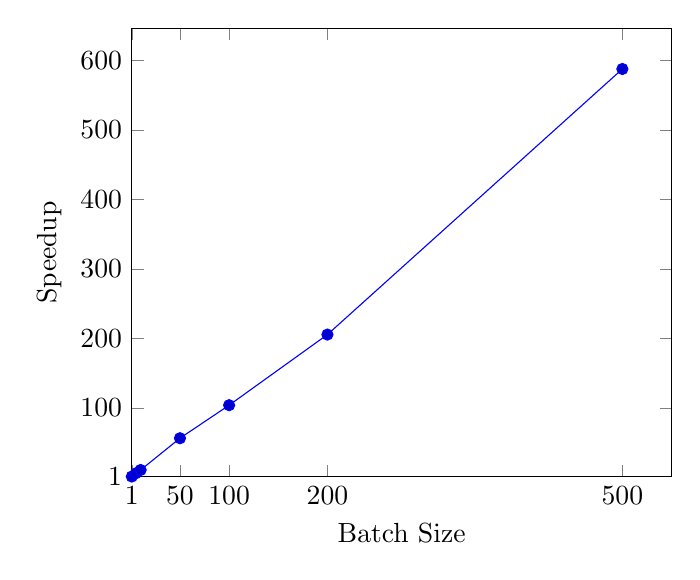
\begin{tikzpicture}
	\begin{axis}
	[xmin=1, ymin=1, ylabel={Speedup}, ytick={1, 100, 200, 300, 400, 500, 600}, xtick={1, 50, 100, 200, 500}, xlabel={Batch Size}]
	\addplot coordinates 
	{(1,1) (5, 5.59) (10, 10.436) (50, 56.178) (100, 103.73) (200, 205.404) (500, 587.764)};
	\end{axis}
	\end{tikzpicture}
	\caption{Speedup for 1 training epoch when training using different batch sizes for PyGPU. Speedup is calculated using the PyGPU model with a batch size of 1 as the reference.}
	\label{gpu-speedup}
\end{figure}

\section{Evaluation Hardware}
The hardware model is evaluated using a ZedBoard equipped with a Zynq-7000 XC7Z020 SoC. The SWM and PyCPU both run on a Intel Core i7-4720HQ CPU. The GPU is an Nvidia GeForce GTX 970M equipped with 6 GB of GDDR5 RAM.

\section{Performance}
One of the most important metrics for an accelerator is runtime performance. 
While this hardware model is primarily focused on training, experiments to determine performance for both training and inference modes have both been conducted and are shown in this section.

\subsection{Training}
The average time for one training epoch has been recorded for each of the neural network models. The result is shown in Figure \ref{train-runtime-res}. This graph shows that the accelerator massively outperforms CPU models. Figure \ref{train-speedup-res} shows the speedup of the models, using PyCPU as a baseline. Notably, the HWM achieves a speedup close to that of the PyGPU model.

\begin{figure}
	\centering
	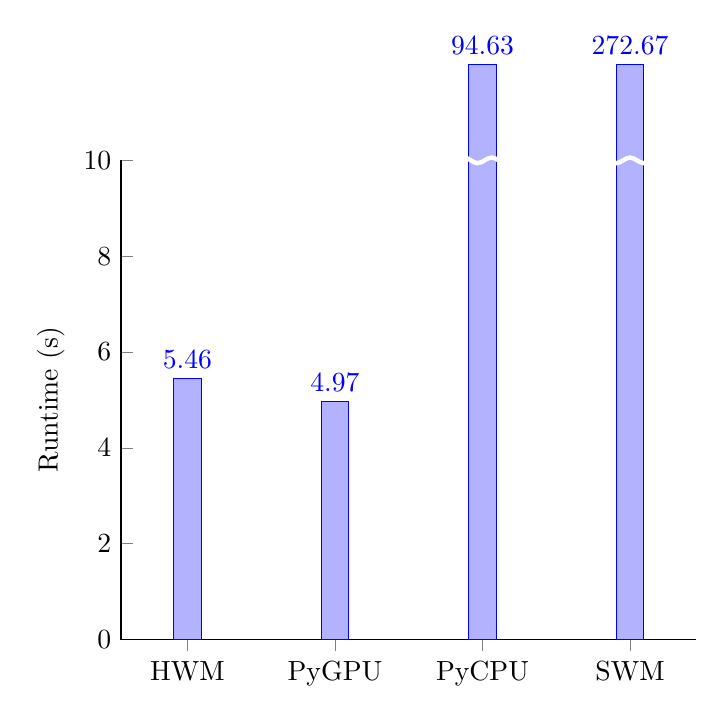
\begin{tikzpicture}
	\begin{axis}[
	ybar,
	width=3.5in,
	enlarge y limits=false,
	enlarge x limits=0.15,
	legend style={at={(0.5,-0.15)},
		anchor=north,legend columns=-1},
	ylabel={Runtime (s)},
	ymin=0,
	ymax=10,
	xmax=SWM,
	restrict y to domain*=0:12, % Cut values off at 14
	visualization depends on=rawy\as\rawy, % Save the unclipped values
	after end axis/.code={ % Draw line indicating break
		\draw [ultra thick, white, decoration={snake, amplitude=1pt}, decorate] (rel axis cs:0.1,1.0) -- (rel axis cs:1.0,1.0);},
	axis lines*=left,
	clip=false,
	nodes near coords={{\pgfmathprintnumber{\rawy}}},
	symbolic x coords={HWM, PyGPU, PyCPU, SWM},
	xtick={data}
	]
	
	\addplot coordinates {(HWM, 5.455)  (PyGPU, 4.9689) (PyCPU, 94.633) (SWM, 272.67)};
	
	\end{axis}
	\end{tikzpicture}
	\caption{Training runtime for various network models}
	\label{train-runtime-res}
\end{figure}

\begin{figure}
	\centering
	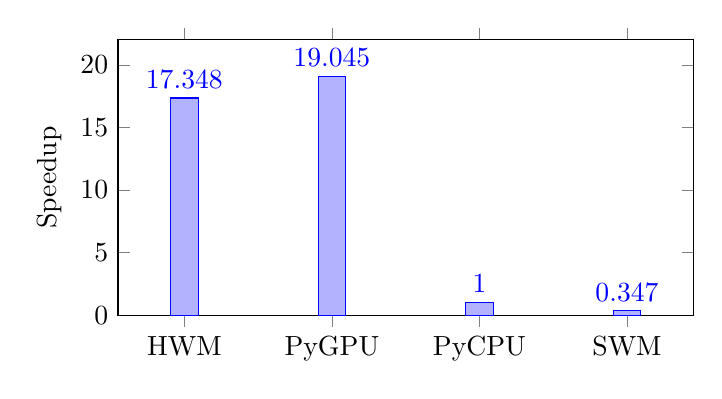
\begin{tikzpicture}
	\begin{axis}[
	ybar,
	width=3.5in,	height=2in,
	enlarge y limits=false,
	enlarge x limits=0.15,
	legend style={at={(0.5,-0.15)},
		anchor=north,legend columns=-1},
	ylabel={Speedup},
	ymin=0,
	ymax=22,
	xmin=HWM,
	xmax=SWM,
	symbolic x coords={HWM, PyGPU, PyCPU, SWM},
	xtick={data},
	scaled y ticks=false,
	nodes near coords,
	nodes near coords style={/pgf/number format/fixed},	
	nodes near coords style={/pgf/number format/precision=3},
	nodes near coords align={vertical}
	]
	
	\addplot coordinates {(HWM, 17.348)  (PyGPU, 19.045) (PyCPU, 1) (SWM, 0.347)};
	
	\end{axis}
	\end{tikzpicture}
	\caption{Training speedup using the PyCPU as a baseline}
	\label{train-speedup-res}
\end{figure}


\subsection{Inference}
Inference performance was also measured for each of the models. The result is shown in Figure \ref{inf-runtime-res}. This graph shows that the accelerator also outperforms CPU models for inference, though falls short of the GPU model. Figure \ref{inf-speedup-res} shows the speedup of the models, using PyCPU as a baseline. The HWM achieves a speedup of 2.282 compared to the PyCPU model.

\begin{figure}
	\centering
	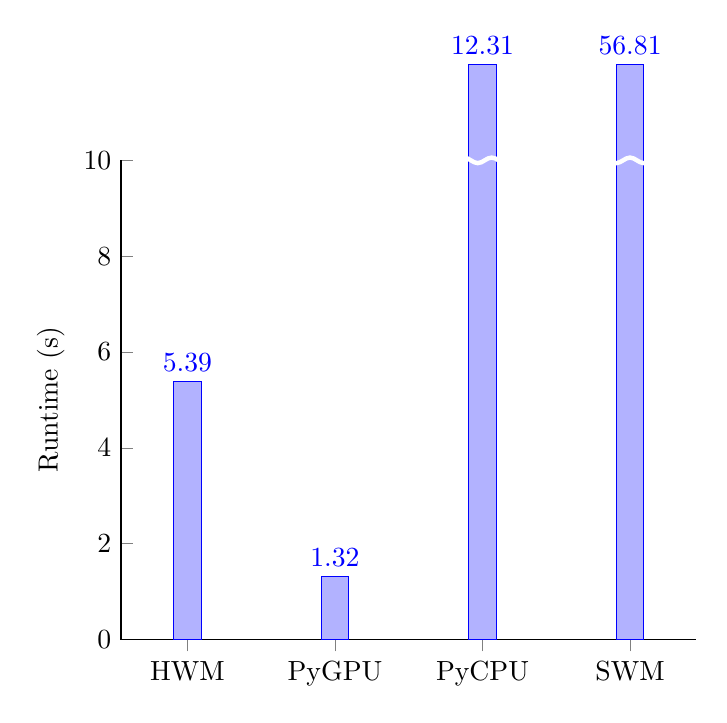
\begin{tikzpicture}
	\begin{axis}[
	ybar,
	width=3.5in,
	enlarge y limits=false,
	enlarge x limits=0.15,
	legend style={at={(0.5,-0.15)},
		anchor=north,legend columns=-1},
	ylabel={Runtime (s)},
	ymin=0,
	ymax=10,
	xmax=SWM,
	restrict y to domain*=0:12, % Cut values off at 14
	visualization depends on=rawy\as\rawy, % Save the unclipped values
	after end axis/.code={ % Draw line indicating break
		\draw [ultra thick, white, decoration={snake, amplitude=1pt}, decorate] (rel axis cs:0.1,1.0) -- (rel axis cs:1.0,1.0);},
	axis lines*=left,
	clip=false,
	symbolic x coords={HWM, PyGPU, PyCPU, SWM}, 
	nodes near coords={{\pgfmathprintnumber{\rawy}}},
	xtick={data}
	]
	
	\addplot 
	coordinates {(HWM, 5.392)  (PyGPU, 1.32) (PyCPU, 12.305) (SWM, 56.808)};
	
	\end{axis}
	\end{tikzpicture}
	\caption{Inference runtime for various network models}
	\label{inf-runtime-res}
\end{figure}

\begin{figure}
	\centering
	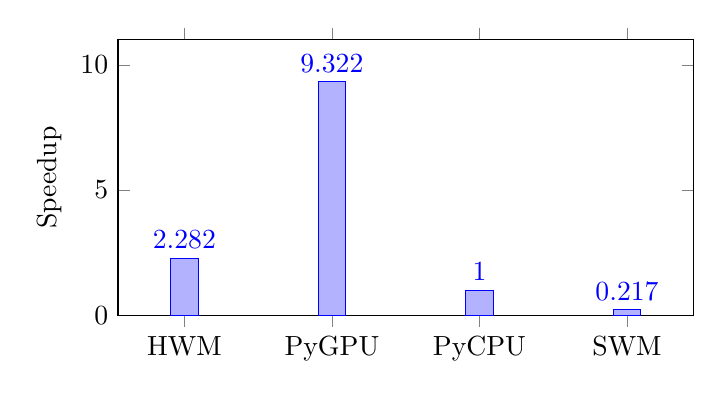
\begin{tikzpicture}
	\begin{axis}[
	ybar,
	height=2in,
	width=3.5in,
	enlarge y limits=false,
	enlarge x limits=0.15,
	legend style={at={(0.5,-0.15)},
		anchor=north,legend columns=-1},
	ylabel={Speedup},
	ymin=0,
	ymax=11,
	xmin=HWM,
	xmax=SWM,
	symbolic x coords={HWM, PyGPU, PyCPU, SWM},
	xtick={data},
	scaled y ticks=false,
	nodes near coords,
	nodes near coords style={/pgf/number format/fixed},	
	nodes near coords style={/pgf/number format/precision=3},
	nodes near coords align={vertical}
	]
	
	\addplot coordinates {(HWM, 2.282)  (PyGPU, 9.322) (PyCPU, 1) (SWM, 0.217)};
	
	\end{axis}
	\end{tikzpicture}
	\caption{Inference speedup using the PyCPU as a baseline}
	\label{inf-speedup-res}
\end{figure}

\subsection{Active/Idle Cycles}
To determine the impact of using MMIO to transfer image data between the PS and the FPGA, active and idle cycles were measured during training and inference. An active cycle is defined as a cycle on the FPGA during which at least one of the layers was computationally active. An idle cycle is thus defined as a non-active cycle. 

An experiment was performed to measure active cycle percentages for the HWM during inference and training. The dataset was the entire MNIST dataset in both cases. The active cycle percentage for inference and training are shown in Table \ref{active-cycle-table}.

\begin{table}
	\centering 
	\begin{tabular}{|c|c|}
		\hline
		& \textbf{Active Cycle Percentage} \\\hline
		Inference & 25.13\% \\\hline 
		Training & 69.20\% \\\hline
	\end{tabular}
	\caption{Active Cycle percentages for inference and training.}
	\label{active-cycle-table}
\end{table}

This experiment was performed to evaluate if the sending of input over MMIO was the bottleneck of the system. As can be clearly seen from the table, the MMIO transfer of training data was indeed the bottleneck. 

\section{Training Accuracy}
This section details the accuracy of the training process using the hardware accelerator. Varying training dataset sizes were chosen as the reduced precision resulted in non-convergent training. As such, the training accuracy experiment conducted modified two variables: the learning rate and the training dataset size. 

The tested learning rates were $2^{-7}$, $2^{-8}$, $2^{-9}$, and $2^{-10}$ (0.0078, 0.0039, 0.00195, and 0.000977). This is because the hardware model performs the learning rate scaling by using bitshifts. The experiments recorded the peak test dataset accuracy during the training process. Note that the test dataset size for each run is 70000 minus the size of the training dataset. The results are shown in Figure \ref{training-accuracy}. In this experiment, the highest test set accuracy, 85.845\%, was achieved with a learning rate of $\eta = 2^{-9}$ and with a dataset of size 4,000. When using the same neural network architecture as the HWM, the SWM converges to 97.6\% test set accuracy.

\begin{figure}
	\centering
	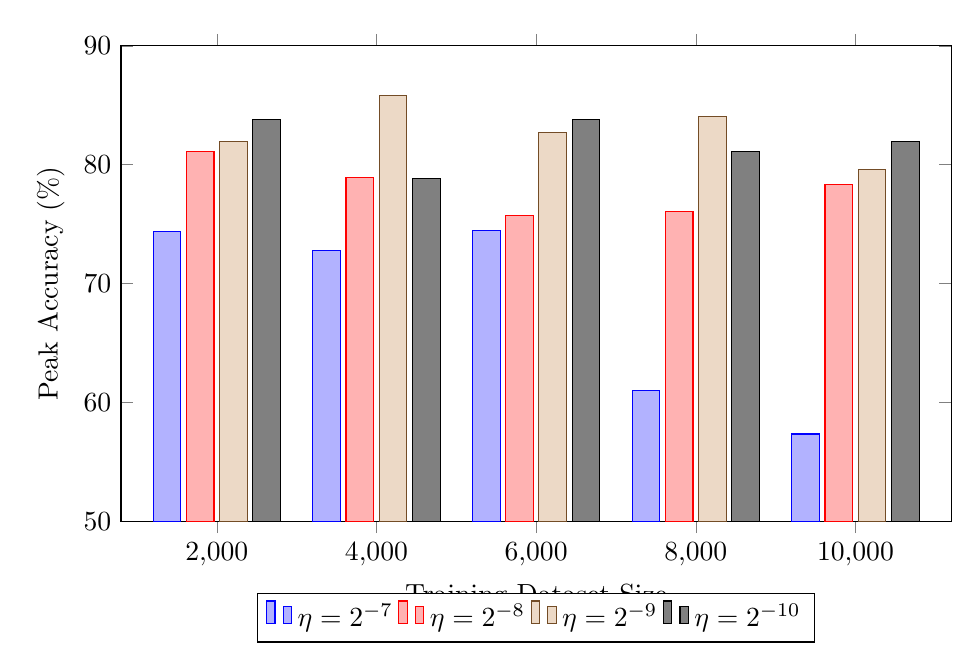
\begin{tikzpicture}
	\begin{axis}[
	ybar,
	height=3in,
	width=\textwidth,
	enlarge y limits=false,
	enlarge x limits=0.15,
	legend style={at={(0.5,-0.15)},
		anchor=north,legend columns=-1},
	ylabel={Peak Accuracy (\%)},
	xlabel={Training Dataset Size},
	ymin=50,
	ymax=90,
	xtick={data},
	scaled y ticks=false,	
	scaled x ticks=false,
	]
	
	\addplot coordinates {(2000, 74.401)  (4000, 72.814) (6000, 74.49) (8000, 61.03) (10000, 57.34)};
	
	\addplot coordinates {(2000, 81.14)  (4000, 78.94) (6000, 75.70) (8000, 76.09) (10000, 78.36)};
	
	\addplot coordinates {(2000, 81.97)  (4000, 85.845) (6000, 82.737) (8000, 84.02) (10000, 79.62)};
	
	\addplot coordinates {(2000, 83.79)  (4000, 78.8) (6000, 83.78) (8000, 81.11) (10000, 81.98)};
	\legend{$\eta = 2^{-7}$, $\eta = 2^{-8}$, $\eta = 2^{-9}$, $\eta = 2^{-10}$}
	\end{axis}
	\end{tikzpicture}
	\caption{Maximum training accuracy reached for various learning rate and training set sizes.}
	\label{training-accuracy}
\end{figure}

\section{Stability of Training}
As previously mentioned, due to the relatively low training precision of 18-bit fixed-point, the training process does not converge to a maximum training accuracy, but rather it will reach a maximum training accuracy, and then accuracy will degrade as precision errors accumulate over the training process. Training statistics for the first 10 epochs of the most optimal training configuration from Figure \ref{training-accuracy} illustrate this phenomenon and are shown in Figure \ref{epoch-by-epoch}.

\begin{figure}
	\centering
	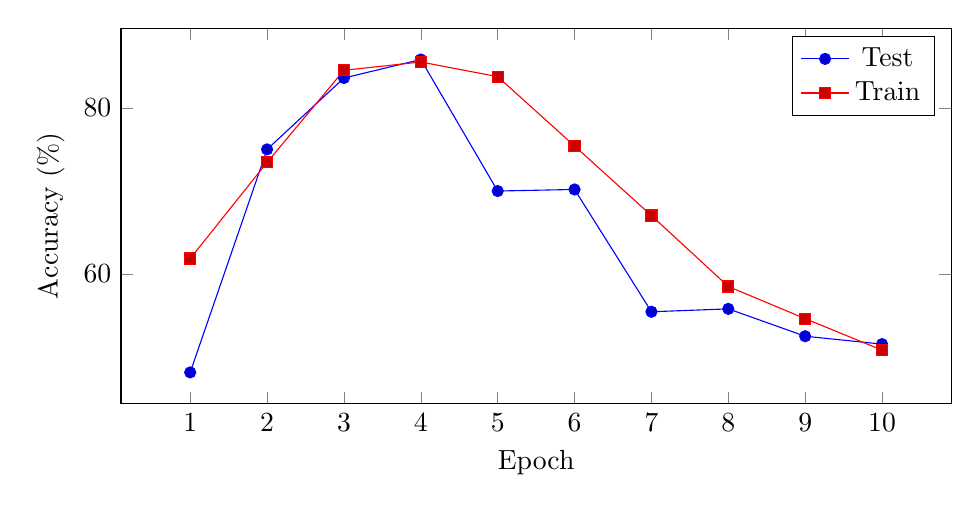
\begin{tikzpicture}
	\begin{axis}[
	ylabel={Accuracy (\%)}, 
	xlabel={Epoch},
	width=\textwidth,
	height=2.5in,
	]
	
	\addplot coordinates 
	{(1, 48.12) (2, 75.012) (3, 83.62) (4, 85.85) (5, 69.99) (6, 70.18) (7, 55.43) (8, 55.78) (9, 52.48) (10, 51.53)};
	\addplot coordinates 	
	{(1, 61.85) (2, 73.45) (3, 84.55) (4, 85.55) (5, 83.78) (6, 75.42) (7, 67.03) (8, 58.48) (9, 54.6) (10, 50.8)};
	
	\legend{Test, Train}
	\end{axis}
	\end{tikzpicture}
	\caption{Epoch-by-epoch training data for an HWM configuration. Clearly visible degradation of accuracy instead of convergence after epoch 4.}
	\label{epoch-by-epoch}
\end{figure}


\section{Implemented Design}
The design implemented for the FPGA is shown in Figure \ref{impl-design}. As expected, the FC1 layer is by and large the most resource intensive, as it utilizes 196 kernels. It is interesting to observe the clustering of individual layer modules, while the interlayer activation buffer for FC0 and FC1 is widely spread out through the FPGA. This would indicate that this interlayer activation buffer was frequently routed to as a midpoint between FC0 and FC1. 

It should be noted that implementation is a non-deterministic process and every design run should result in a slightly different implemented design. However, general trends for routing of the design tend to  persist throughout multiple runs, despite the non-determism of the placing and routing algorithms.

\begin{figure}
	\centering
	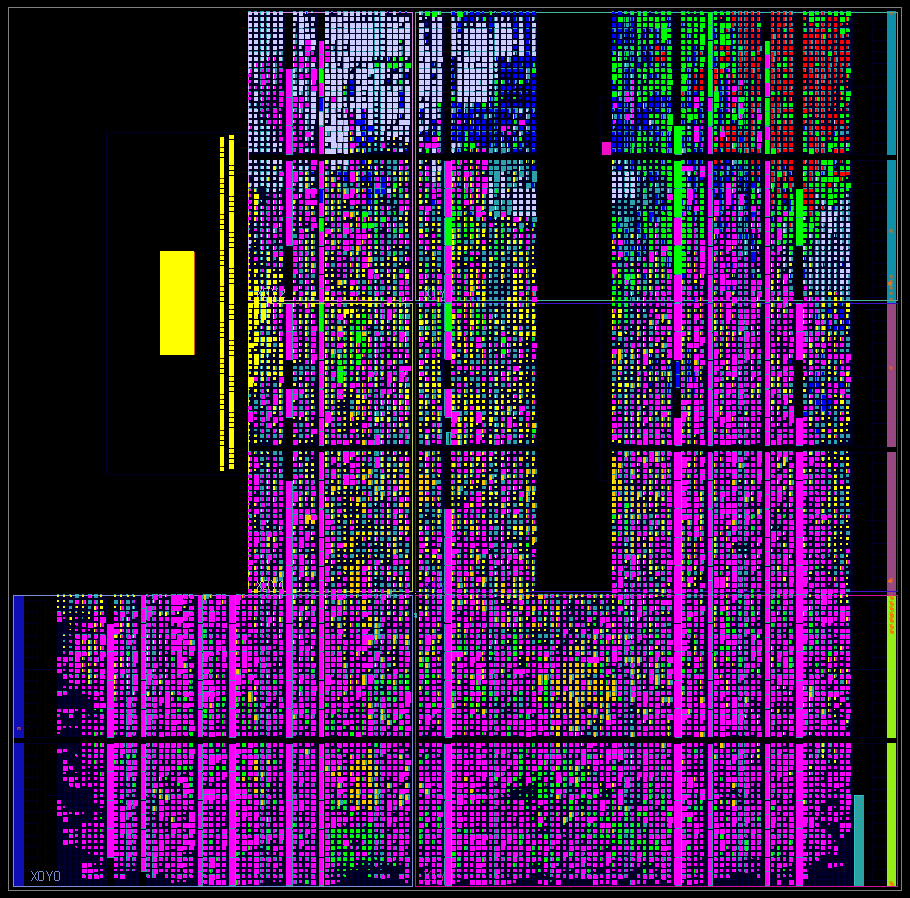
\includegraphics[width=\textwidth]{figures/impl_design}
	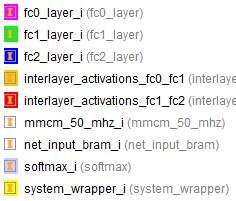
\includegraphics{figures/impl_design_legend}
	\caption{The implemented design of the hardware model}
	\label{impl-design}
\end{figure}

\subsection{Resource Usage, Power, and Timing}
The resource usage of the hardware model is shown in Table \ref{resource-usage}. As can be seen, the DSP slice is the scarcest resource, with LUTs and BRAMs also heavily being used.  Overall, high utilization of the FPGA resources was intentional, trying to optimize the performance of the accelerator as much as possible.
\begin{table}
	\centering 
	\begin{tabular}{|l|l|l|c|}
	\hline 
	\textbf{Resource} & \textbf{Utilization} & \textbf{Available} & \textbf{Utilization \%} \\\hline 
	LUT & 41132 & 53200 & 77.32		\\\hline
	FF & 54097 & 106400 & 50.84 \\\hline 
	BRAM & 107.5 & 140 & 76.79 \\\hline 
	DSP & 215 & 220 & 97.73 \\\hline	
	\end{tabular}
\caption{Resource usage of the implemented design}
\label{resource-usage}
\end{table}

According to the Vivado report, the total on-chip power of the design is 2.798 Watts. While this number is reported with `Low' confidence by Vivado, this wattage is far lower than typical GPU power consumptions. Power measurements have not been made for the internal GPU during these experiments, though measurements using the Torch framework were made and reported GPU average power at 94.19 Watts while performing training using the AlexNet architecture. The power measurements were performed with an Nvidia Tesla K20M GPU with 5 GB of GDDR5 SDRAM, a top-of-the-line GPU \cite{xinbochen2016}. This is several magnitudes higher than the FPGA based solution in this thesis. 

The implemented design for the hardware model is clocked at a frequency of 50 MHz. Placement and routing are both able to successfully complete with no timing violations. There was no need to improve frequency because the current performance bottleneck of this design stems from data transfer over the AXI bus and not from FPGA computational speed.                                  %Chapter 6
\chapter{Analysis}\label{analysis}

\section{Allocating Computationl Kernels for Performance}
\subsection{Allocating Based on Only Forward Pass Analysis}
When computing an optimal allocation of kernels to the fully-connected layers, it was enough to account only for the forward pass. This is because in the backward pass, there are 2 times the kernel is used, during previous layer neuron gradient calculation, and during weight gradient calculation. In each case, the amount of multiplications is equal to the sum of the fan-ins of all the neurons. For the forward pass, every neuron receives an input from every neuron in the previous layer, so the amount of MACs will be:
\begin{align}
MACs = \text{\#previous layer neurons} \times \text{\#current layer neurons} \label{macs}
\end{align}

For the backward pass, each backpropagated neuron gradient to a previous layer requires an MAC on all the neurons in the current layer. This must be done for each neuron in the previous layer, thus the total amount of MACs for backpropagating neuron gradients is also equivalent to Equation \ref{macs}.

For computing all the weight gradients in a layer, every weight for every neuron must be multiplied by a gradient. Each neuron in the current layer will have a \# previous layer neurons weights, as that is the fan-in for each neuron. Thus, there same amount of multiplications is also equal to the expresion in Equation \ref{macs}.

The backward pass also has a weight updating step, however, this uses bitshifts and not DSP slices to multiply the weight gradient by the learning rate. As such, the backward pass in this model uses exactly twice the amount of multiplications as the forward pass, so the optimal allocation of kernels is optimal for both the forward and backward pass. Note however, that even if the update step used multiplication, the amount of extra multiplications would be 1 for every weight, which would still be a multiple of the amount of multiplciations in the forward pass.

\subsection{Distribution of the Kernels}
Table \ref{macs-per-layer} shows the fan-in, number of neurons, and thus the number of MACs per layer during the forward pass. 
\begin{table}
	\centering
	\begin{tabular}{|l|l|l|l|}
		\hline
		Layer & Fan-in per Neuron & \# Neurons & MACs \\\hline 
		FC0 & 784  & 98 & 76832 \\\hline 
		FC1 & 98 & 64 & 6272 \\\hline 
		FC2 & 64 & 10 & 640 \\\hline
	\end{tabular}
	\caption{MACs per layer during the forward pass}
	\label{macs-per-layer}
\end{table}

Furthermore, recall that a kernel operates on only 1 neuron at a time. Therefore, the amount of kernels allocated should be either a multiple or a factor of the amount of neurons such that work can be evenly distributed across the kernels. Given the 220 DSP slices on the FPGA, this becomes an optimization problem such that the amount of time for each layer to finish computing their outputs should be roughly the same. This would allow for pipelined input processing if offline training for large batch-sizes were to be implemented.

FC0 has 120.05 times more MACs than FC2. FC1 has 9.8 times more MACs than FC2. To balance runtime per layer, FC0 should then have roughly 120.05 times more DSPs than FC2 and so on. Using this information, we can write an equation for the amount of MACs and use substitution to come up with an ideal allocation scheme if allocate partial DSPs and ignore the fact that kernels work on 1 neuron at a time.
\begin{align}
	\text{DSP}_{FC0} &= 120.05 {DSP}_{FC2} \label{mac-1}\\	
	\text{DSP}_{FC1} &= 12.25 {DSP}_{FC2} \label{mac-2}\\
	\text{\# DSPs} &= 220 = \text{DSP}_{FC0} + \text{DSP}_{FC1} + \text{DSP}_{FC2} \label{mac-3}\\	
	\intertext{Substituting into equation \ref{mac-3} using equations \ref{mac-1} and \ref{mac-2}:}\\
	220 &= 120.05 {DSP}_{FC2} + 12.25  {DSP}_{FC2} +  {DSP}_{FC2} \\
	220 &= 133.3 {DSP}_{FC2}\\ 
	{DSP}_{FC2} &= 1.65 \label{mac-4}\\
	\intertext{Substituting the result from \ref{mac-4} into equations \ref{mac-1} and \ref{mac-2}:}
	\text{DSP}_{FC0} &= 120.05 \times 1.65 = 198.08\label{mac-5}\\	
	\text{DSP}_{FC1} &= 12.25 \times 1.65 = 20.21\label{mac-6}	
\end{align}
Thus if the 220 DSPs could be divided up ignoring all previous restrictions, the DSPs should be allocated according to Equations \ref{mac-4}, \ref{mac-5} and \ref{mac-6}. However, this is not possible, and DSPs are indivisible and the amount of kernels per layer should be a factor or multiple of the number of neurons, but it provides an maximum upper bound for performance.

Starting with layer FC0, which has 98 neurons, we should delegate 196 kernels. This is quite close to the optimal 198.08 computed above, thus layer FC0 should be allocated 196 kernels, which is 98.9\% of the maximum upper bound. Continuing to layer FC1, which has 64 neurons, the optimal allocation is 20.21. The two closest factors of 64 would be 16 and 32. Choosing 32 is not an option because there would not be enough kernels available, so only 16 kernels are allocated to layer FC1, roughly 79\% of maximum upper bound for performance. Finally, layer FC1, with 10 neurons, rounding down and allocating 1 kernel would result in only 60.6\% of the upper bound performance. Since we have freed up a few kernels from rounding down in FC0 and FC1, FC2 is thus allocated 2 kernels, which allows it to finish faster than the optimally balanced latency for the 3 layers.

The final allocation of kernels is shown in Table \ref{dsp-allocat}. A pipelined solution is only as fast as its slowest step. Since FC1 is the farthest away from the optimal upper bound, this solution performs at 79\% of the theoretical upper bound. It is worth re-mentioning that this upper bound is infeasible for this solution since it assumes DSPs as divisible and that kernels can arbitrarily switched from neuron to neuron, which would require finer-parallelism than what is supported, as this solution utilizes parallelism at the neuron-level. Also note that since 214 of the 220 DSPs are used, the softmax layer will also be able to use a DSP for calculation of the exponential function.

\begin{table}
	\centering 
	\begin{tabular}{|l|l|}
		\hline 
		Layer & \# Kernels \\\hline
		FC0 & 196 \\\hline
		FC1 & 16 \\\hline
		FC2 & 2	\\\hline
		Total & 214	\\\hline
	\end{tabular}
	\caption{Kernel allocation between the fully-connected layers.}
	\label{dsp-allocat}
\end{table}

\section{Cycle Analysis}
\todo[inline]{math for cycle analysis, done already on a powerpoint before}

\section{Improving Performance}
As was shown in Table \ref{active-cycle-table} of the results section, the active cycle percentage for training is only 69.20\%. Thus the first step to improve runtime performance would be to make data available for the FPGA to process faster. A suggested approach would be to use DRAM to stream data to the FPGA as done in other projects such as the neural network inference hardware accelerator proposed by Qiao et. al \cite{qiao}.

If an active cycle percentage of near 100\% can be achieved from doing this, the next step to would be to optimize performance on the FPGA. The quickest route to doing this would be to improve the clock frequency. The design was clocked at a relatively low-frequency since it was not the bottleneck for performance. As such, the clock frequency was not investigated heavily during the design of the FPGA architecture, since improving this clock frequency would only increase the amount of time that the layers in the FPGA spend idling.

\section{Granularity for Neural Network Computation}
A key difference between training using this accelerator and training using GPUs is that this accelerator uses a much more fine-grained level of parallelism. While GPUs use data-level parallelism, this design uses neuron-level parallelism. Some attempts  have been made to implement finer-level parallelism training on GPUs by Jiang et. al, though only yielded modest improvements of 1.58 to 2.19 times the speedup \cite{fine-grained-gpu}. 

As a result, if one were to use the PyGPU solution to perform online training, then the GPU is 2.95 times slower than the CPU solution, which was 17.35 times slower than the hardware model (results in \cite[inline]{Experiment results appendix}). Therefore, for online training, using fine-grained parallelism at the neuron level is the only place to find speedup, as data-level parallelism is not possible during online training where the batch size is only 1.

\section{Ideal Learning Rate vs. Precision}
One of the key intricacies in optimizing hyperparameters for the training process was balancing an ideal learning rate against increased precision error. Normally one need not think about precision when choosing a learning rate. However, in this accelerator, choosing what perhaps would be a more ideal learning rate might actually induce higher training error if it is too small since a smaller learning rate means fewer bits of gradient data are kept. For this project, this is compounded even further by the general notion that online training performs best with smaller learning rates. 

For example, a learning rate of 0.001 results in a much better solution than a learning rate of 0.016 when a batch size of 1 is used for the implemented network architecture. However, the smaller in the implemented accelerator, this would mean an additional 4 bitshifts to the right when updating the weights. This results in a weight update that will have 4 fewer bits of information. In this project, the best training solution was found using 9 bitshifts to the right, or a learning rate of 0.00195. The weight gradients in this project are of number format Q1.17. Shifting this to the right 9 bits results in a Q1.8 number. This means that each and every weight update in the network only have 8 bits of information.

\paragraph{Vanishing Gradient Problem}
To add on even further to the aforementioned loss of information is that many of the gradients are already quite small. This is largely in part to a phenomenon referred to as the vanishing gradient problem. The vanishing gradient problem in neural networks refers to the fact that as one backpropagates further and further through the network, the gradients become smaller and smaller. To illustrate this point, the distributions of non-zero gradients in the implemented network has been plotted in Figure \todo[inline]{Plot gradient distribution by layer}. Thus, as the gradients become smaller and smaller, they also become harder to represent, and when you are already losing many bits of information due to the learning rate, the vanishing gradient problem exacerbates the precision-induced error during training even more.

\section{Potential Solutions for the Lack of Precision}
As 18-bit fixed-point computation has been shown to be too imprecise to perform training on this network, potential solutions to this problem should be observed. It is the author's opinion that future accelerators for the training of neural networks would be best implemeneted by using 32-bit floating point as was done in the F-CNN accelerator by Zhao et. al \cite{FCNN}. 

However, if 32-bit floating point is infeasible, or if accuracy is to be traded off for improved speed, area, and storage of weights, then investigations into designing accelerators using 16-bit or 24-bit floating-point computation could be made.

If the architecture must use fixed point, then the author would suggest first investigating 32-bit fixed-point computation with varying radices. If storage restrictions permit and the design performs multiplications using DSP slices, then a maximum of 36 bits would be supported for completing a multiplication using 2 DSPs in 1 cycle. This stems from the fact that 18 bits is the maximum width for one of the ports in a DSP-multiply. Otherwise, multiplication could also be a multi-cycle computation to trade off time for improved precision.

\section{Weight Storage}
The implemented neural network was specifically designed such that the weights and weight gradients could fit in the BRAM. Since 76.79\% of the BRAM was utilized, the implemented network is representative of what architectures may be supported in BRAM as it comes close to hitting the upper limit of network size that can be supported entirely using BRAM. For networks larger than the implemented neural network for this thesis, other solutions such as a streaming weight and weight gradient datapath to DRAM would be required. 

In addition, since the precision of the weight and weight gradients in this project proved to be inadequate for convergence to a local optimum during training, it should be noted that increasing precision would also increase BRAM utilization. This network would be able to use a maximum of 23-bits of precision for the weights while still fitting into BRAM at roughly 98.12\% utilization. If more bits are needed for successful training then the network architecture would have to be made smaller or the hardware architecture would need to use a streaming datapath solution.
                                 	%Chapter 7
\chapter{Discussion}\label{discussion}
\section{Overall Performance}
Regarding the performance, the accelerator has outperformed all compared CPU benchmarks. It performs online training with a speedup of 17.35 compared to the PyTorch CPU model. Considering how the PyTorch GPU achieved a 19.05 speedup using a batch size of 50, the accelerator was nearly able to keep pace. Furthermore, the GPU model does not use fine-level parallelism, so the accelerator achieves the highest speedup of all models for training with a batch size of 1.

\section{Finely-Grained Parallelism}
Training of neural networks in today's world is done almost exclusively using GPUs and occasionally using CPUs. This is a stark contrast compared to inference, for which many different chips such as Google's TPU have been developed \cite{TPU}. However, as this thesis has shown, for neural network training problems that do not have vast amount of data parallelism available, there is no highly optimized solution. As such, the accelerator developed during the process of this thesis shows a massive potential for this side of training since it takes advantage of the finely-grained parallelism available at the neuron-level, something not done by options available in today's world.

\section{Limitations}
\subsection{Precision}
Precision is a major limitation of training for the current design. It is the reason why the training process is not able to smoothly converge to a local optimum. This results in contradicting desires to have more bits of information available in weights gradients while at the same time having a low learning rate.

\subsection{Data Transfer Rate}
Another major limitation of this work is the method of transferring training data by using a memory-mapped interface between the PS to the FPGA. This approach was used for convenience, however, as the FPGA active cycle results from Table \ref{active-cycle-table} showed, this approach is inefficient and became the largest bottleneck of performance for the design.

\section{Future Work}
While the potential for application-specific hardware accelerators training has been demonstrated in this thesis, there is a lot of potential for future work to improve the project.

\paragraph{Increased Precision}
As was demonstrated in the results section, training a neural network requires high precision computation. This is especially true for deeper neural networks as a result of the vanishing gradient problem. Therefore, increasing the precision, either via changing to floating point or using more bits in fixed point would be a great improvement.

\paragraph{Larger Batch Sizes}
Online training is only applicable to certain datasets. While the usefulness of an accelerator for online training has been shown, there are also many datasets that converge faster by using a larger batch size and offline training. In addition, a larger batch size provides a more accurate gradient of the actual loss function of the training set. 

Since the amount of data-level parallelism increases with the batch size, it becomes increasingly harder to compete with the performance of GPUs. Furthermore, a solution to storing activations in memory to compute the backward must be designed. That being said, using a larger batch size would also open up the possibility to taking advantage of data-level parallelism and using an array of training accelerators. In such a setup, both data-level and neuron-level parallelism would be working together.

\paragraph{Additional Layer Types}
This design only implemented the fully-connected and softmax layer types. There are many other types of layers for neural networks, and this project could be expanded by implementing other layer types such as convolutional or pooling layers, which are  frequently used in image recognition.

\paragraph{Backward Pass for Biases}
In the interest of time and since the input data is already fairly normalized, only the backward pass for weights was computed. A rather quick improvement to the project would be to implement the backward pass for biases, so that the network architecture could be applied to non-normalized datasets as well. The gradient for a bias is simply the gradient of the net, as it is added directly to the net. Therefore, the bias gradients are already known in the hardware, and all that would need to be done is adding BRAMs for the biases and slightly modify the update phase to update the biases.

\paragraph{Additional Activation Functions}
In both the software and hardware models for this project, the ReLU function was chosen specifically due to its computational simplicity, quick convergence during training, and its ability to converge to strong local optima. That being said, there are still many other activation functions in the realm of neural networks that also achieve strong training results. As the dataset and network architecture changes, so may the the most optimal activation function. Other activations functions such as the sigmoid function, leaky ReLU, hyperbolic tangent, and many others may be preferred to ReLU under certain circumstances. These functions would require extra hardware support though, and thus would require more computational resources to implement. As a result, one should expect that the performance of the accelerator would not be quite so high as with the ReLU activation function.

\paragraph{Implement Streaming DDR Interface for FPGA}
Adding a streaming data interface for training data would reduce the amount of cycles during which the FPGA idles. This would be a strong improvement for performance. Adding a streaming data DDR interface for weights and activations would allow networks with larger footprints to be supported by the hardware model. Both of these modifications would be an overall improvement to the model.

\paragraph{Generated HDL for a Pre-Specified Network Architecture}
As one of the design goals was to be modular, if the streaming data interface were to be implemented, then it would be feasible to define a network architecture in a configuration file and create a program to generate HDL files for that network architecture. This would allow for a flexible, modular, FPGA-based framework that could implement any type of network, so long as the layer-types of that network were supported.
                                 	%Chapter 8
\chapter{Conclusion}                                 	%Chapter 9
\appendix
\chapter{Stuff}

This appendix is full of stuff ...                                 %Appendix
\chapter{Hardware Model Code}\label{app:hw}
This appendix contains the SystemVerilog code used to implement the hardware accelerator. Display statements have been omitted as they serve no functional purpose to the implementation nor is there any particular insight to be gained from them. They may of course still be viewed at the GitHub repository. Note that some style has been modified make code fit on the page.


\lstset{basicstyle=\footnotesize\ttfamily, captionpos=t}
\section{Source Files}
\subsection{sys\_defs.vh}
\lstinputlisting[language=SystemVerilog, upquote=true]{HardwareCode/sys_defs.vh}
\pagebreak

\subsection{neural\_net\_top.sv}
\lstinputlisting[language=SystemVerilog, upquote=true]{HardwareCode/neural_net_top.sv}
\pagebreak

\subsection{fc0\_layer.sv}
\lstinputlisting[language=SystemVerilog, upquote=true]{HardwareCode/fc0_layer.sv}
\pagebreak

\subsection{fc0\_weight\_bram\_controller.sv}
\lstinputlisting[language=SystemVerilog, upquote=true]{HardwareCode/fc0_weight_bram_controller.sv}
\pagebreak

\subsection{fc\_kernel.sv}
\lstinputlisting[language=SystemVerilog, upquote=true]{HardwareCode/fc_kernel.sv}
\pagebreak

\subsection{fc\_scheduler.sv}
\lstinputlisting[language=SystemVerilog, upquote=true]{HardwareCode/fc_scheduler.sv}
\pagebreak

\subsection{interlayer\_activation\_buffer.sv}
\lstinputlisting[language=SystemVerilog, upquote=true]{HardwareCode/interlayer_activation_buffer.sv}
\pagebreak

\subsection{fc1\_layer.sv}
\lstinputlisting[language=SystemVerilog, upquote=true]{HardwareCode/fc1_layer.sv}
\pagebreak

\subsection{previous\_layer\_gradient\_adder.sv}
\lstinputlisting[language=SystemVerilog, upquote=true]{HardwareCode/previous_layer_gradient_adder.sv}
\pagebreak

\subsection{fc1\_weight\_bram\_controller.sv}
\lstinputlisting[language=SystemVerilog, upquote=true]{HardwareCode/fc1_weight_bram_controller.sv}
\pagebreak


\subsection{fc2\_layer.sv}
\lstinputlisting[language=SystemVerilog, upquote=true]{HardwareCode/fc2_layer.sv}
\pagebreak

\subsection{fc2\_weight\_bram\_controller.sv}
\lstinputlisting[language=SystemVerilog, upquote=true]{HardwareCode/fc2_weight_bram_controller.sv}
\pagebreak

\subsection{softmax.sv}
\lstinputlisting[language=SystemVerilog, upquote=true]{HardwareCode/softmax.sv}
\pagebreak

\section{Testbenches}
\subsection{neural\_net\_top\_tb.sv}
\lstinputlisting[language=SystemVerilog, upquote=true]{HardwareCode/neural_net_top_tb.sv}
\pagebreak

\subsection{softmax\_tb.sv}
\lstinputlisting[language=SystemVerilog, upquote=true]{HardwareCode/softmax_tb.sv}
\pagebreak

\subsection{fc1\_scheduler\_tb.sv}
\lstinputlisting[language=SystemVerilog, upquote=true]{HardwareCode/fc1_scheduler_tb.sv}
\pagebreak

\subsection{fc1\_layer\_tb.sv}
\lstinputlisting[language=SystemVerilog, upquote=true]{HardwareCode/fc1_layer_tb.sv}
\pagebreak






                                 %Appendix
\chapter{Processing System Code}\label{app:ps}
This appendix contains the source code for the programs that run on the PS. It should be noted that \textit{inference\_only.c} and \textit{train.c} are quite similar. This code was written in C and cross-compiled for ARM.
\section{train.c}
\lstinputlisting[language=C, upquote=true]{PSCode/train.c}
\pagebreak

\section{inference\_only.c}
\lstinputlisting[language=C, upquote=true]{PSCode/inference_only.c}
\pagebreak

\section{parse\_mnist.c}
\lstinputlisting[language=C, upquote=true]{PSCode/parse_mnist.c}
\pagebreak                                 %Appendix 
\chapter{Hardware Testing Code}\label{app:hw-test}
This Appendix contains the code that was use to verify the simulated output of the hardware model. This code was written in Python.

\section{fpga\_forward\_backward\_pass\_test.py}
\lstinputlisting[language=Python, upquote=true]{HWTestCode/fpga_forward_backward_pass_test.py}
\pagebreak                                 %Appendix 
\chapter{Weight Generation}\label{app:wg}
This appendix contains the code that was used to generate the Xilinx coefficient files to initialize the weight BRAMs in the hardware model using He Initialization. This code was written in Python.

\section{weight\_coeff.py}
\lstinputlisting[language=Python, upquote=true]{WeightGenCode/weight_coeff.py}
\pagebreak                                 %Appendix 
\chapter{Software Model}\label{app:sw}
This appendix contains the code that was used to implement the software model for this project. The software model was written in C++.
\section{Header Files}

\subsection{net.h}
\lstinputlisting[language=C++, upquote=true]{SWModel/src/net.h}
\pagebreak


\subsection{layer.h}
\lstinputlisting[language=C++, upquote=true]{SWModel/src/layer.h}
\pagebreak


\subsection{convolutional.h}
\lstinputlisting[language=C++, upquote=true]{SWModel/src/convolutional.h}
\pagebreak


\subsection{fullyconnected.h}
\lstinputlisting[language=C++, upquote=true]{SWModel/src/fullyconnected.h}
\pagebreak

\subsection{pooling.h}
\lstinputlisting[language=C++, upquote=true]{SWModel/src/pooling.h}
\pagebreak


\subsection{neuron.h}
\lstinputlisting[language=C++, upquote=true]{SWModel/src/neuron.h}
\pagebreak


\subsection{parse\_data.h}
\lstinputlisting[language=C++, upquote=true]{SWModel/src/parse_data.h}
\pagebreak


\section{Source Files}

\subsection{main.cpp}
\lstinputlisting[language=C++, upquote=true]{SWModel/src/main.cpp}
\pagebreak


\subsection{net.cpp}
\lstinputlisting[language=C++, upquote=true]{SWModel/src/net.cpp}
\pagebreak

\subsection{convolutional.cpp}
\lstinputlisting[language=C++, upquote=true]{SWModel/src/convolutional.cpp}
\pagebreak

\subsection{fullyconncted.cpp}
\lstinputlisting[language=C++, upquote=true]{SWModel/src/fullyconnected.cpp}
\pagebreak

\subsection{pooling.cpp}
\lstinputlisting[language=C++, upquote=true]{SWModel/src/pooling.cpp}
\pagebreak

\subsection{neuron.cpp}
\lstinputlisting[language=C++, upquote=true]{SWModel/src/neuron.cpp}
\pagebreak

\subsection{parse\_data.cpp}
\lstinputlisting[language=C++, upquote=true]{SWModel/src/parse_data.cpp}
\pagebreak


\section{Testing Files}
\subsection{gradient\_check\_test.cpp}
\lstinputlisting[language=C++, upquote=true]{SWModel/test/gradient_check_test.cpp}
\pagebreak

\subsection{conv\_test.cpp}
\lstinputlisting[language=C++, upquote=true]{SWModel/test/conv_test.cpp}
\pagebreak


\subsection{fullyconnected\_test.cpp}
\lstinputlisting[language=C++, upquote=true]{SWModel/test/fullyconnected_test.cpp}
\pagebreak


\subsection{neuron\_test.cpp}
\lstinputlisting[language=C++, upquote=true]{SWModel/test/neuron_test.cpp}
\pagebreak
                                 %Appendix 
\chapter{PyTorch Model}
This appendix contains the code for the PyTorch version of the implemented neural network. This code was written in Python.

\section{mnist\_model.py}
\lstinputlisting[language=Python, upquote=true]{PyTorchModel/mnist_model.py}
\pagebreak

\section{parse\_data.py}
\lstinputlisting[language=Python, upquote=true]{PyTorchModel/parse_data.py}
\pagebreak
%-----------
% Backmatter
%-----------
\backmatter
\chaptermark{Bibliography}
\renewcommand{\sectionmark}[1]{\markright{#1}}
\sectionmark{Bibliography}
\addcontentsline{toc}{chapter}{Bibliography}        %Force addition of Bibliography to TO

\bibliographystyle{alpha}                           %Use alpha codes for references
\bibliography{References}                           %Bibliography file called
\end{document}
% % % EOF % % %